\chapter{Experimental Results}\label{chap:results}

In this chapter we present experimental results.
All experiments are run under 12.04 Ubuntu Linux on an ASUS K46C laptop,
which has four Intel Core i5-3317U CPU and 3.8GiB RAM.
\todo[inline]{how do I say later I found out I need more RAM so switch to another computer?}

Various algorithms (including the path equilibration algorithm) for solving
the traffic assignment problem has already been implemented by Olga Perederieieva, the co-supervisor of this project.
The algorithms are written in C++, compiled by the g++ compiler using the `-O3' optimization flag.

\todo[inline]{Bellman was only SP algorithm available, all the results in this chapter are based on newly developed code.}

All timed results are measured for a complete run of traffic assignment.
All solutions will use $10^{-6}$ as the relative gap for the stopping criterion.

\todo[inline]{see top of page 28 Andrea fix}
\section{Road networks}

Table~\ref{table:problemdata} shows the road networks used for this project, the network details are retrieved from \citet{ProblemData}.
The table has an extra column showing the minimum number of iterations the path equilibration algorithm takes to solve the networks.
Compared to other networks in the table,
Anaheim, Barcelona and Winnipeg are small networks.
Chicago Sketch is a medium sized network that is part of the Chicago Regional network.
Berlin Center is a medium sized network.
Philadelphia and Chicago Regional are two large networks that have over a million number of O-D pairs.

\todo[inline]{see bottom of page 28 Andrea fix}
\begin{table}[H]
    \centering
    \begin{tabular*}{\textwidth}{@{\extracolsep{\fill}} l|c|rrrr|r} \toprule
        Network         & Category & Nodes & Arcs & Zones & O-D pairs & Iterations \\ \midrule
        %SiouxFalls     & 24    & 24   & 528     & 76    \\
        Anaheim         & small & $378$   & $  914$    & $38      $ & $1{,}406   $    & 10  \\
        Barcelona       & small & $910$ & $ 2{,}522$ & $110     $ & $7{,}922   $    & 27  \\
        Winnipeg        & small & $905$ & $ 2{,}836$ & $147     $ & $4{,}344   $    & 126 \\
        Chicago Sketch   & medium & $546$   & $ 2{,}950$ & $387     $ & $93{,}135  $    & 25  \\ 
        Berlin Center   & medium & $ 12{,}116$ & $ 28{,}376$ & $865$ & $49{,}688   $    & 23 \\
        Philadelphia    & large & $11{,}864$ & $40{,}004$ & $1{,}525$ & $1{,}149{,}795$ & 81  \\
        Chicago Regional & large & $11{,}192$ & $39{,}018$ & $1{,}790$ & $2{,}296{,}227$ & 152 \\
        \bottomrule
    \end{tabular*}
    \caption{Network Problem Data}
    \label{table:problemdata}
\end{table}

\section{Results on priority queues} \label{sec:pq_results}
In this section we study different priority queues discussed in Section~\ref{sec:pq_implementation}.
The priority queues are used in Dijkstra's algorithm on the Winnipeg and Chicago Sketch networks.
The results are shown in Figure~\ref{fig:pq_runtime2} and~\ref{fig:pq_runtime}.
The exact numerical results can be found in Appendix~\ref{appendix:pq_results}.

On both networks, 
$\langle$priority\_queue$\rangle$ has the best performance and the Binomial heap has the worst performance.
Skew heap has the best performance among the six heap implementations from the Boost library.
Fibonacci heap has worse performance compared to some of the other implementations despite of its $O(1)$ Insert and Increase-Key operation.
$\langle$set$\rangle$ is significantly slower than $\langle$priority\_queue$\rangle$.

\todo[inline]{see page 29 Andrea fix, clarify results discussion}

\begin{figure}[H]
    \centering
    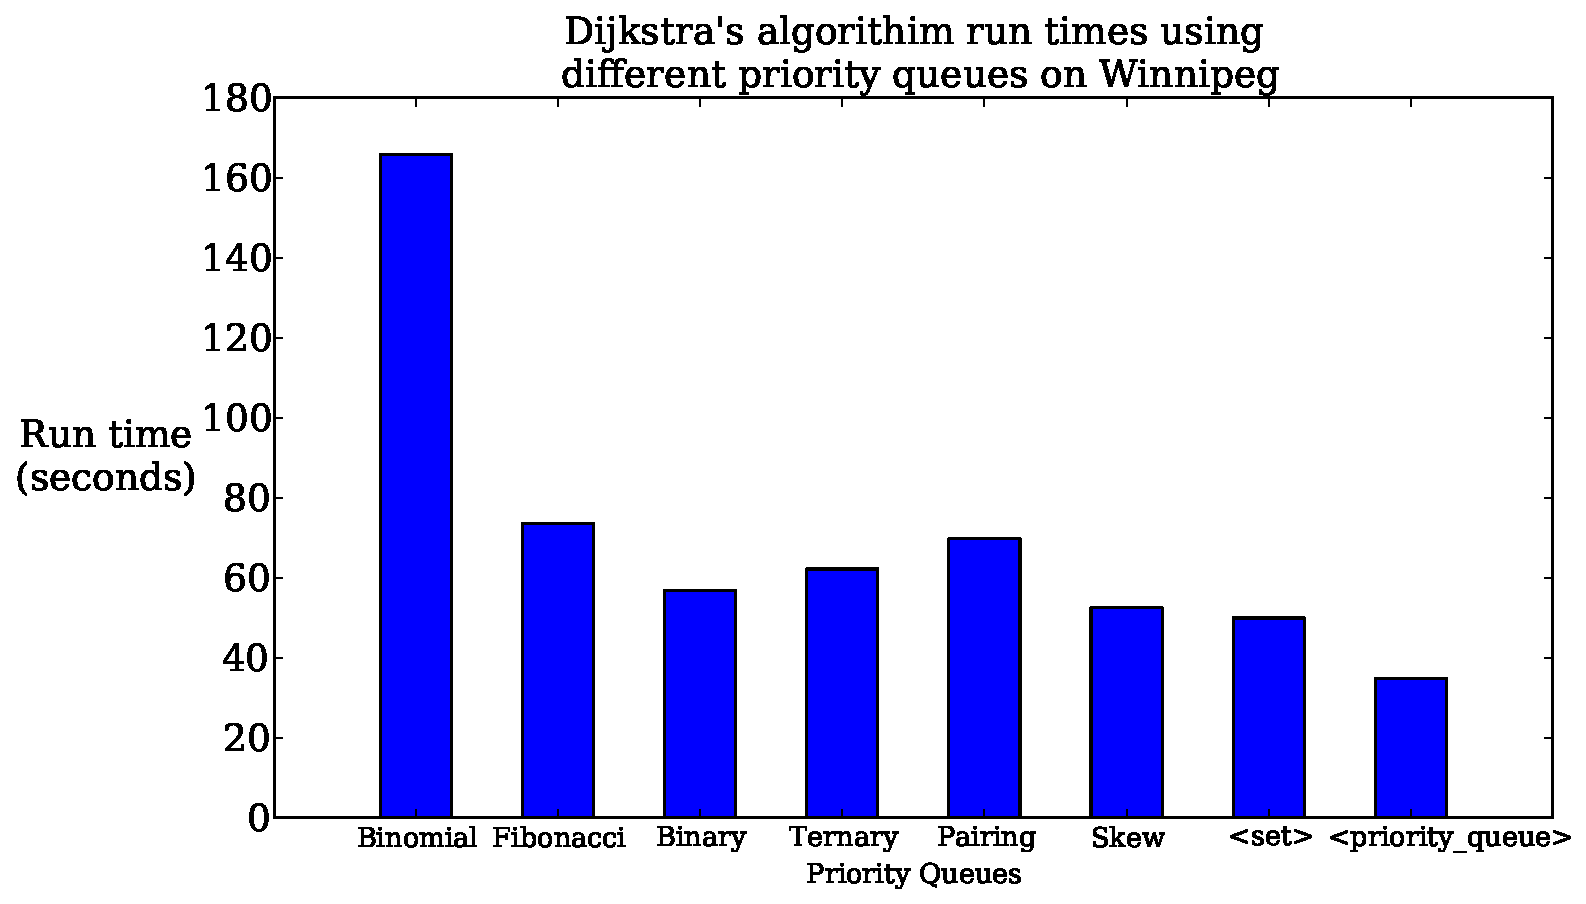
\includegraphics[page=1, width=\textwidth, height=.4\textheight]{img/pq_runtime}
    \caption{Full traffic assignment run times using Dijkstra's algorithm with different priority queues on Winnipeg, with a total number of $547{,}344$ shortest paths solved.}
    \label{fig:pq_runtime2}
\end{figure}
\begin{figure}[H]
    \centering
    \includegraphics[page=2, width=\textwidth, height=.4\textheight]{img/pq_runtime}
    \caption{Full traffic assignment run times using Dijkstra's algorithm with different priority queues on Chicago Sketch, with a total number of $2{,}328{,}375$ shortest paths solved.}
    \label{fig:pq_runtime}
\end{figure}

\section{Results on shortest path algorithms} \label{sec:allresults}
In Section~\ref{sec:pq_results} we have identified  $\langle$priority\_queue$\rangle$ to be the most suitable (efficient) data structure to be used in Dijkstra's algorithm
Now we use $\langle$priority\_queue$\rangle$, implement and test the following algorithms:
\begin{itemize}
        \item Bellman-Ford-Moore algorithm (existing),
        \item Dijkstra's algorithm,
        \item Bidirectional Dijkstra's algorithm,
        \item A* search,
        \item Bidirectional A* search.
\end{itemize}
%Therefore we use $\langle$priority\_queue$\rangle$ from the C++ standard template library and implement Dijkstra's algorithms and A* search, as well as their bidirectional versions.
Figure~\ref{fig:allresults} shows the performance of the mentioned algorithms on the Anaheim, Barcelona, Winnipeg and Chicago Sketch networks
(see Appendix~\ref{appendix:sp_results} for exact numerical results).
The networks are spaced out on the horizontal axis to show their relative sizes, i.e.\ the number of O-D pairs.

Bellman-Ford-Moore algorithm has the worst performance while the A* search has the best performance on all networks.
The bidirectional versions of Dijkstra's algorithm and A* search are more than twice slower than their unidirectional versions.

\begin{figure}[H]
    \centering
    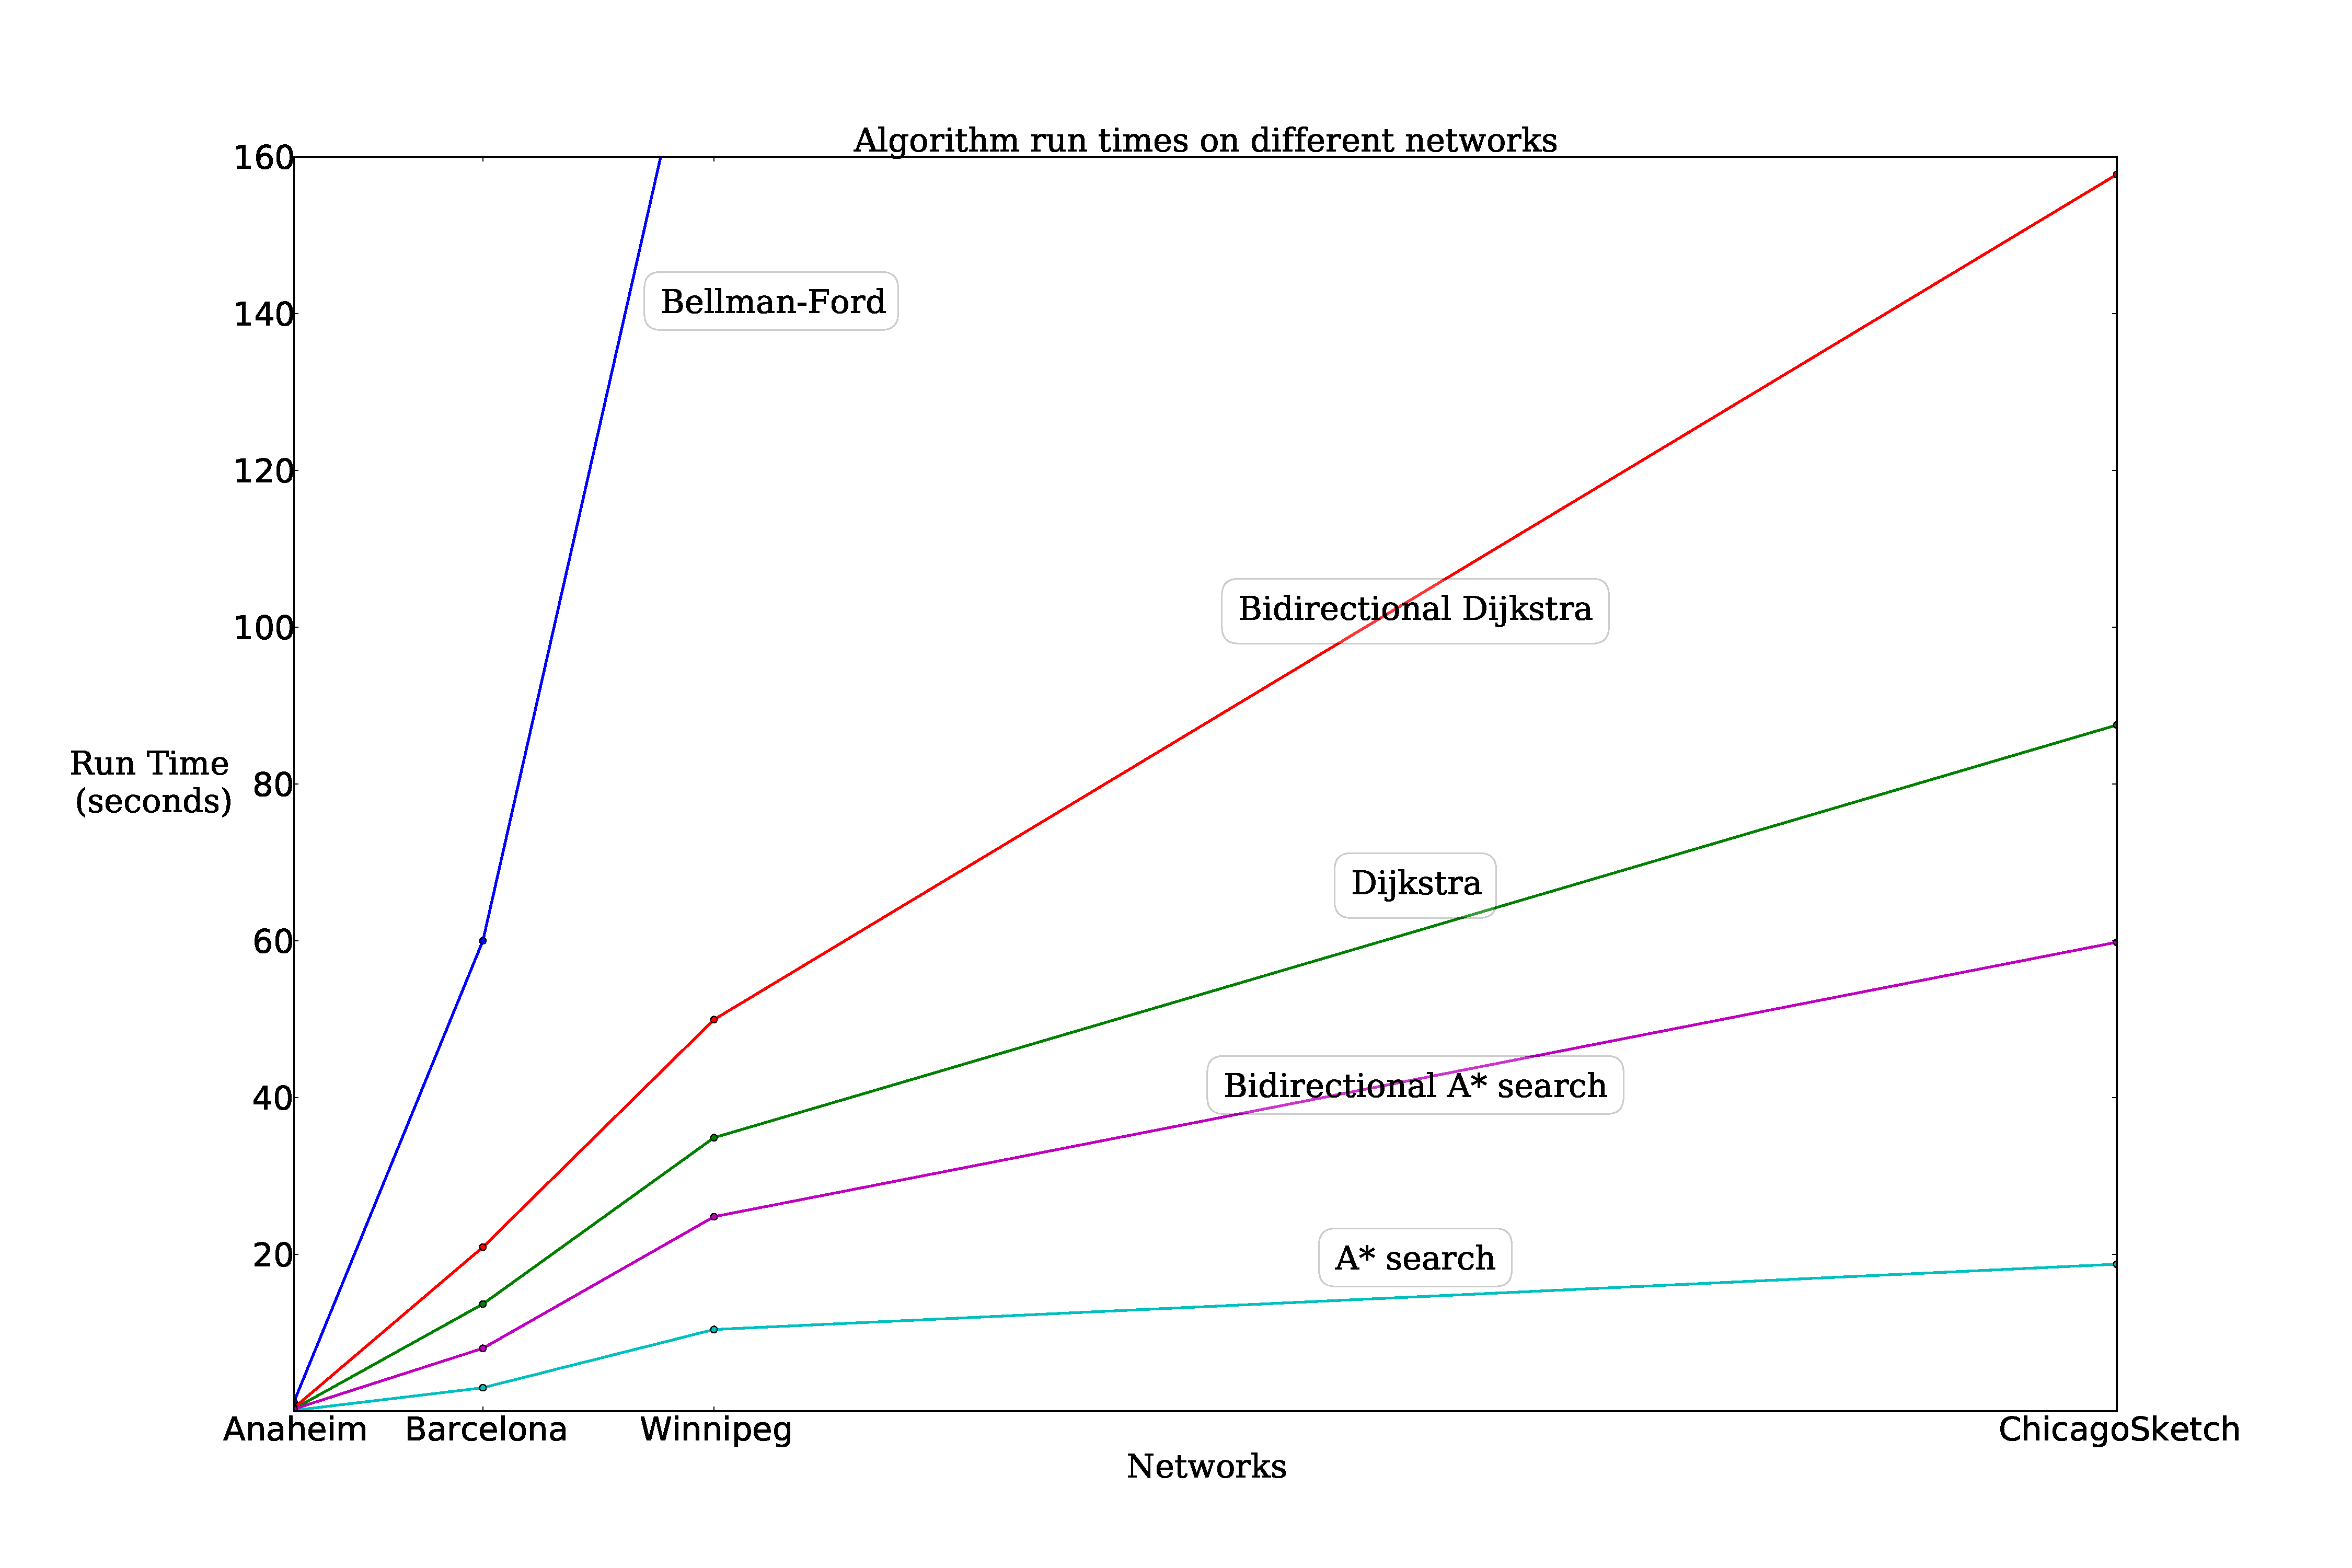
\includegraphics[width=\textwidth]{img/runtime}
    \caption{Run time performances of different algorithms on different networks}
    \label{fig:allresults}
\end{figure}
\todo[inline]{bigger axis label and remove line to different shapes}

\section{Results on avoiding shortest path calculations}
In Section~\ref{sec:allresults} we have identified A* search to be the most suitable (efficient) algorithm for solving the point-to-point shortest path problem.
In this section, we consider avoiding shortest path calculations in the iterative path equilibration algorithm discussed in Section~\ref{section:avoid}.
A* search is used to generate results for this section.

As mentioned in Section~\ref{section:avoid},
in order to apply shortest path avoiding strategies,
we need to first prove that most of the shortest paths do not change often.

Figure~\ref{fig:sp_change} shows 
the histogram for the number of times the shortest path for an O-D pair changed 0,1,2,\ldots times on the Chicago Sketch network.
It shows out of 26 iterations,
the percentage of O-D pairs that changed their shortest path once, twice, three times etc.
The figure shows that 60\% of O-D pairs have not changed their shortest path after the initial iteration,
and 16\% of O-D pairs changed their shortest path only once.
This means that after the first iterations,
the algorithm spends most of its time changing only a dozen of O-D pairs' shortest path out of $93{,}135$.
From these observations,
it is assured that run time can be reduced if we avoid shortest path calculations on the paths that do not change between iterations.

\begin{figure}[H]
    \centering
    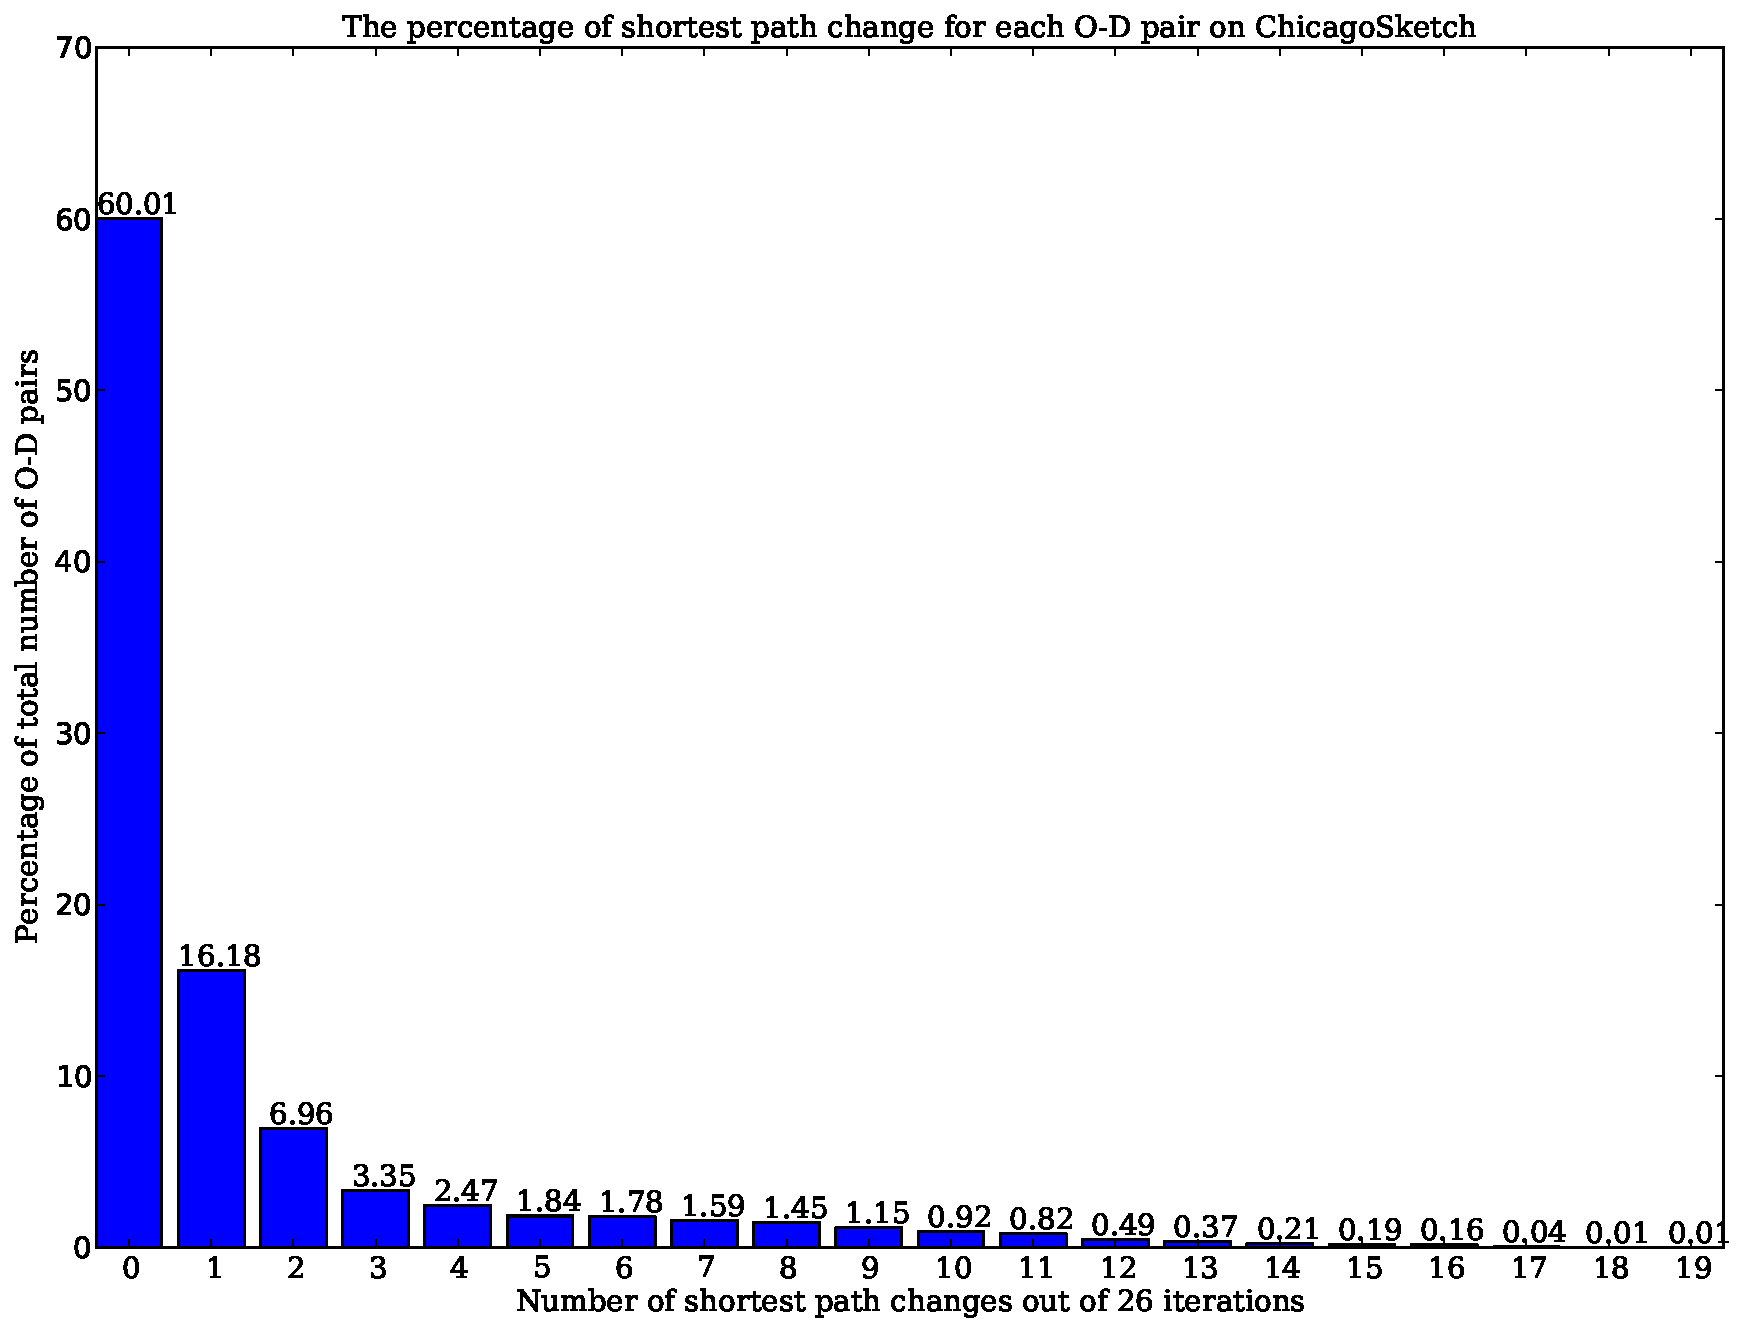
\includegraphics[height=.5\textheight]{img/sp_change}
    \caption{The percentage of shortest path change for each O-D pair out of 26 iterations for Chicago Sketch}
    \label{fig:sp_change}
\end{figure}
\todo{change title and axis label}

We now present the strategy of avoiding a pre-defined number of shortest path calculations for each O-D pair if the previous two iterations result in the identical shortest path trees.
The results are shown in Figure~\ref{fig:skip_n},
where the strategy is experimented on the Terrassa and Chicago Sketch network.
On the Terrassa network,
we choose to avoid the next 15, 25, 50, 100 and 200 iterations of shortest path calculations if the previous two are the same.
And on the Chicago Sketch network,
we choose to avoid the next 5, 10, 15 and 20 iterations.
The strategy worked well on the Terrassa network,
where run time is decreased by half for all of the chosen number of avoiding iterations.
Due to small size of the network,
the run time is not affected even though the total number of iterations increased to 563 when calculations are avoided by 200 iterations.
The strategy also worked well on the Chicago Sketch network.
Skipping 5 iterations resulted the same 26 iterations and the run time is decreased by 4 seconds.
Run times are still reduced in cases where there is an increase in total number of iterations.

\begin{figure}[H]
    \centering
    \begin{subfigure}{.5\textwidth}
        \centering
        \includegraphics[page=3,width=\textwidth]{img/random_time}
        \caption{Terrassa network}
        \label{fig:terrassa_skip_n}
    \end{subfigure}%
    \begin{subfigure}{.5\textwidth}
        \centering
        \includegraphics[page=4,width=\textwidth]{img/random_time}
        \caption{Chicago Sketch network}
        \label{fig:chicago_skip_n}
    \end{subfigure}
    \caption{Run time for avoiding shortest path calculations if the previous two iteration did not change}
    \label{fig:skip_n}
\end{figure}

The other strategy is to skip the next shortest path calculation randomly.
%The advantage of this strategy is that it does not need the number of iterations it will compute,
%but the disadvantage is that the run time may vary between different runs.
Figure~\ref{fig:terrassa_random_n} shows the results on the Terrassa network, probabilities of 0.3, 0.4, 0.5, 0.6 and 0.7 for skipping the next shortest path calculation.
The strategy reduced the run time quite significantly for all probabilities,
especially 0.5.
Figure~\ref{fig:chicago_random_n} shows effect of the same strategy on the Chicago Sketch network.
This time all run times are reduced slightly, with 0.4 having the most reduction.

\begin{figure}[H]
    \centering
    \begin{subfigure}{.5\textwidth}
        \centering
        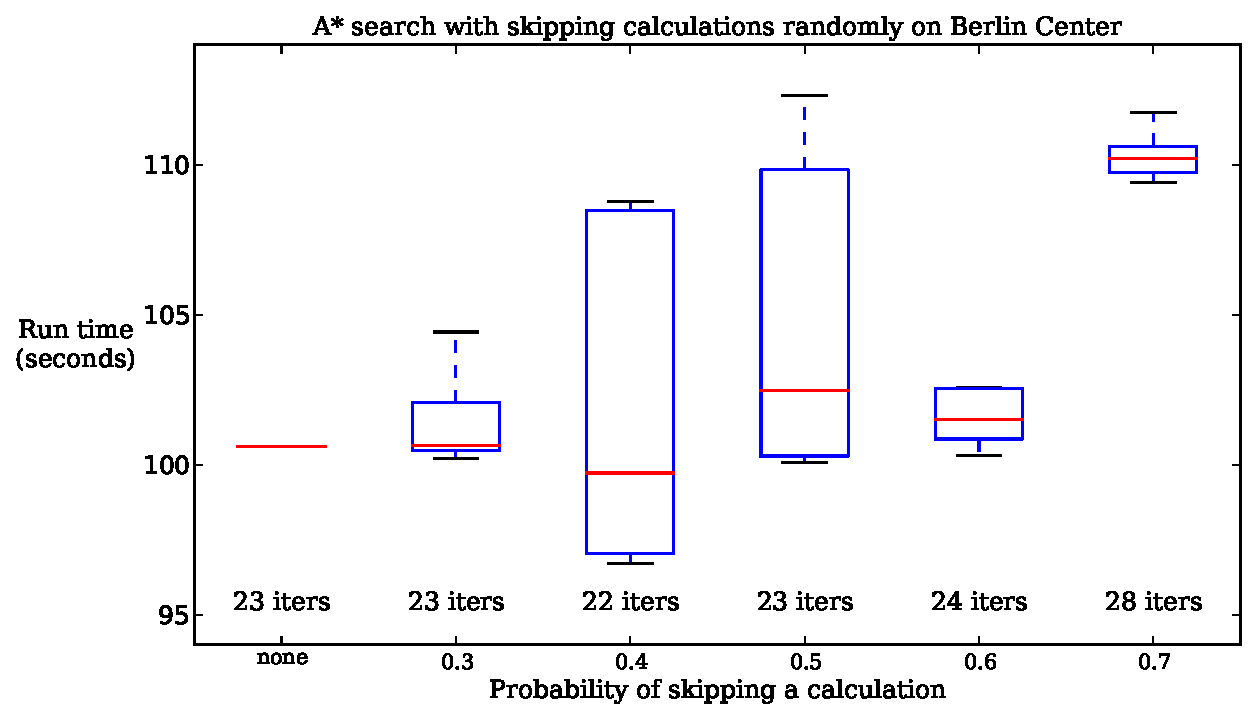
\includegraphics[page=1,width=\textwidth]{img/random_time}
        \caption{Terrassa network}
        \label{fig:terrassa_random_n}
    \end{subfigure}%
    \begin{subfigure}{.5\textwidth}
        \centering
        \includegraphics[page=2,width=\textwidth]{img/random_time}
        \caption{ChicagoSketch network}
        \label{fig:chicago_random_n}
    \end{subfigure}
    \caption{Run time for skipping shortest path calculations randomly}
    \label{fig:random_n}
\end{figure}

The random strategy can be used before knowing the total number of iterations the path equilibration algorithm going to produce,
Since only small networks have been tested so far,
we now present the random strategy on the Philadelphia and Chicago Regional networks, where they have over a million number of O-D pairs.
The run time comparisons are shown in Table~\ref{table:runtime_large_network},
where the random skipping strategy uses 50\% probability to skip a shortest path calculation.
The strategy has a 25\% and 27\% run time improvement on the Philadelphia and Chicago Regional networks respectively.

\begin{table}[H]
    \begin{tabular*}{\textwidth}{@{\extracolsep{\fill}} l | c c}
        & Philadelphia & Chicago Regional \\ \midrule
        A* search & 7.69 hours & 33.26 hours \\ 
        A* search with 50\% random skipping & 5.75 hours & 24.18 hours\\
    \end{tabular*}
    \caption{Run time of A* search and the randomly skipping strategy on Philadelphia and Chicago Regional network}
    \label{table:runtime_large_network}
\end{table}

\todo[inline]{see page 34 Andrea fix}
